% !TEX root = ./../main.tex
\chapter{Molecular description of the process}
%Introduzione a seguito dei risultati con la metadinamica: run unbiased con PW striped, random11, random 12 e POPC

\section{Water dragging}
%Trascinamento delle PW nelle varie salse

%	WPatchedComparison		WRPComparison
\begin{figure}[]
	\center
	\subfloat[]{
		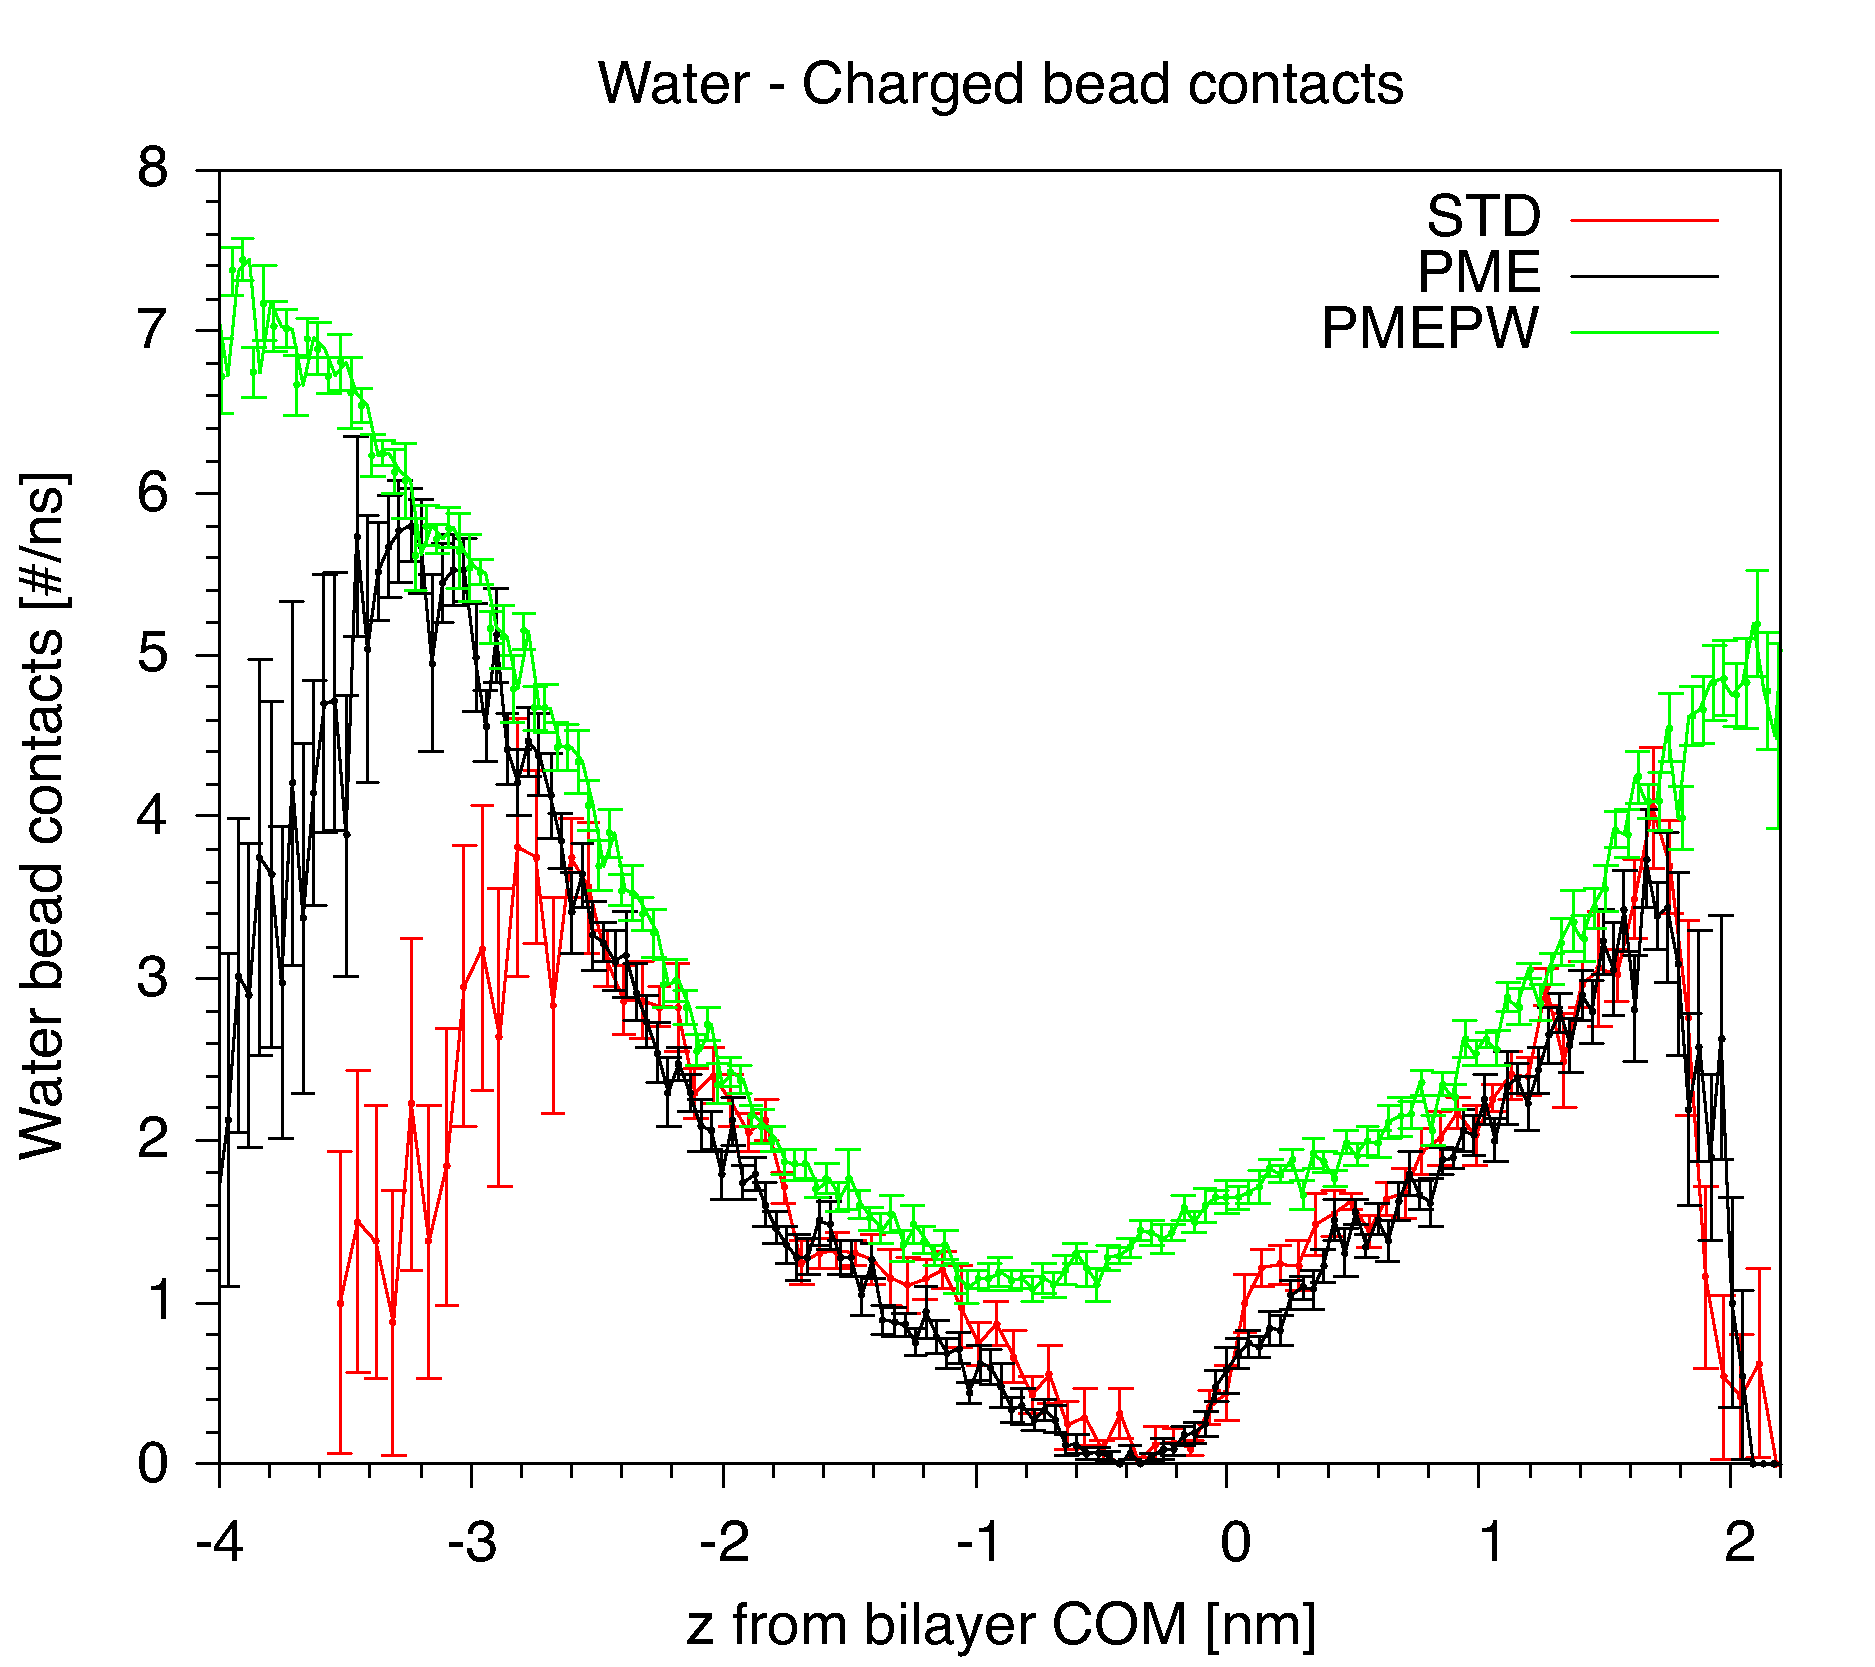
\includegraphics[width=0.5\textwidth]{./img/results/WPatchedComparison}
	}%
	\subfloat[]{
		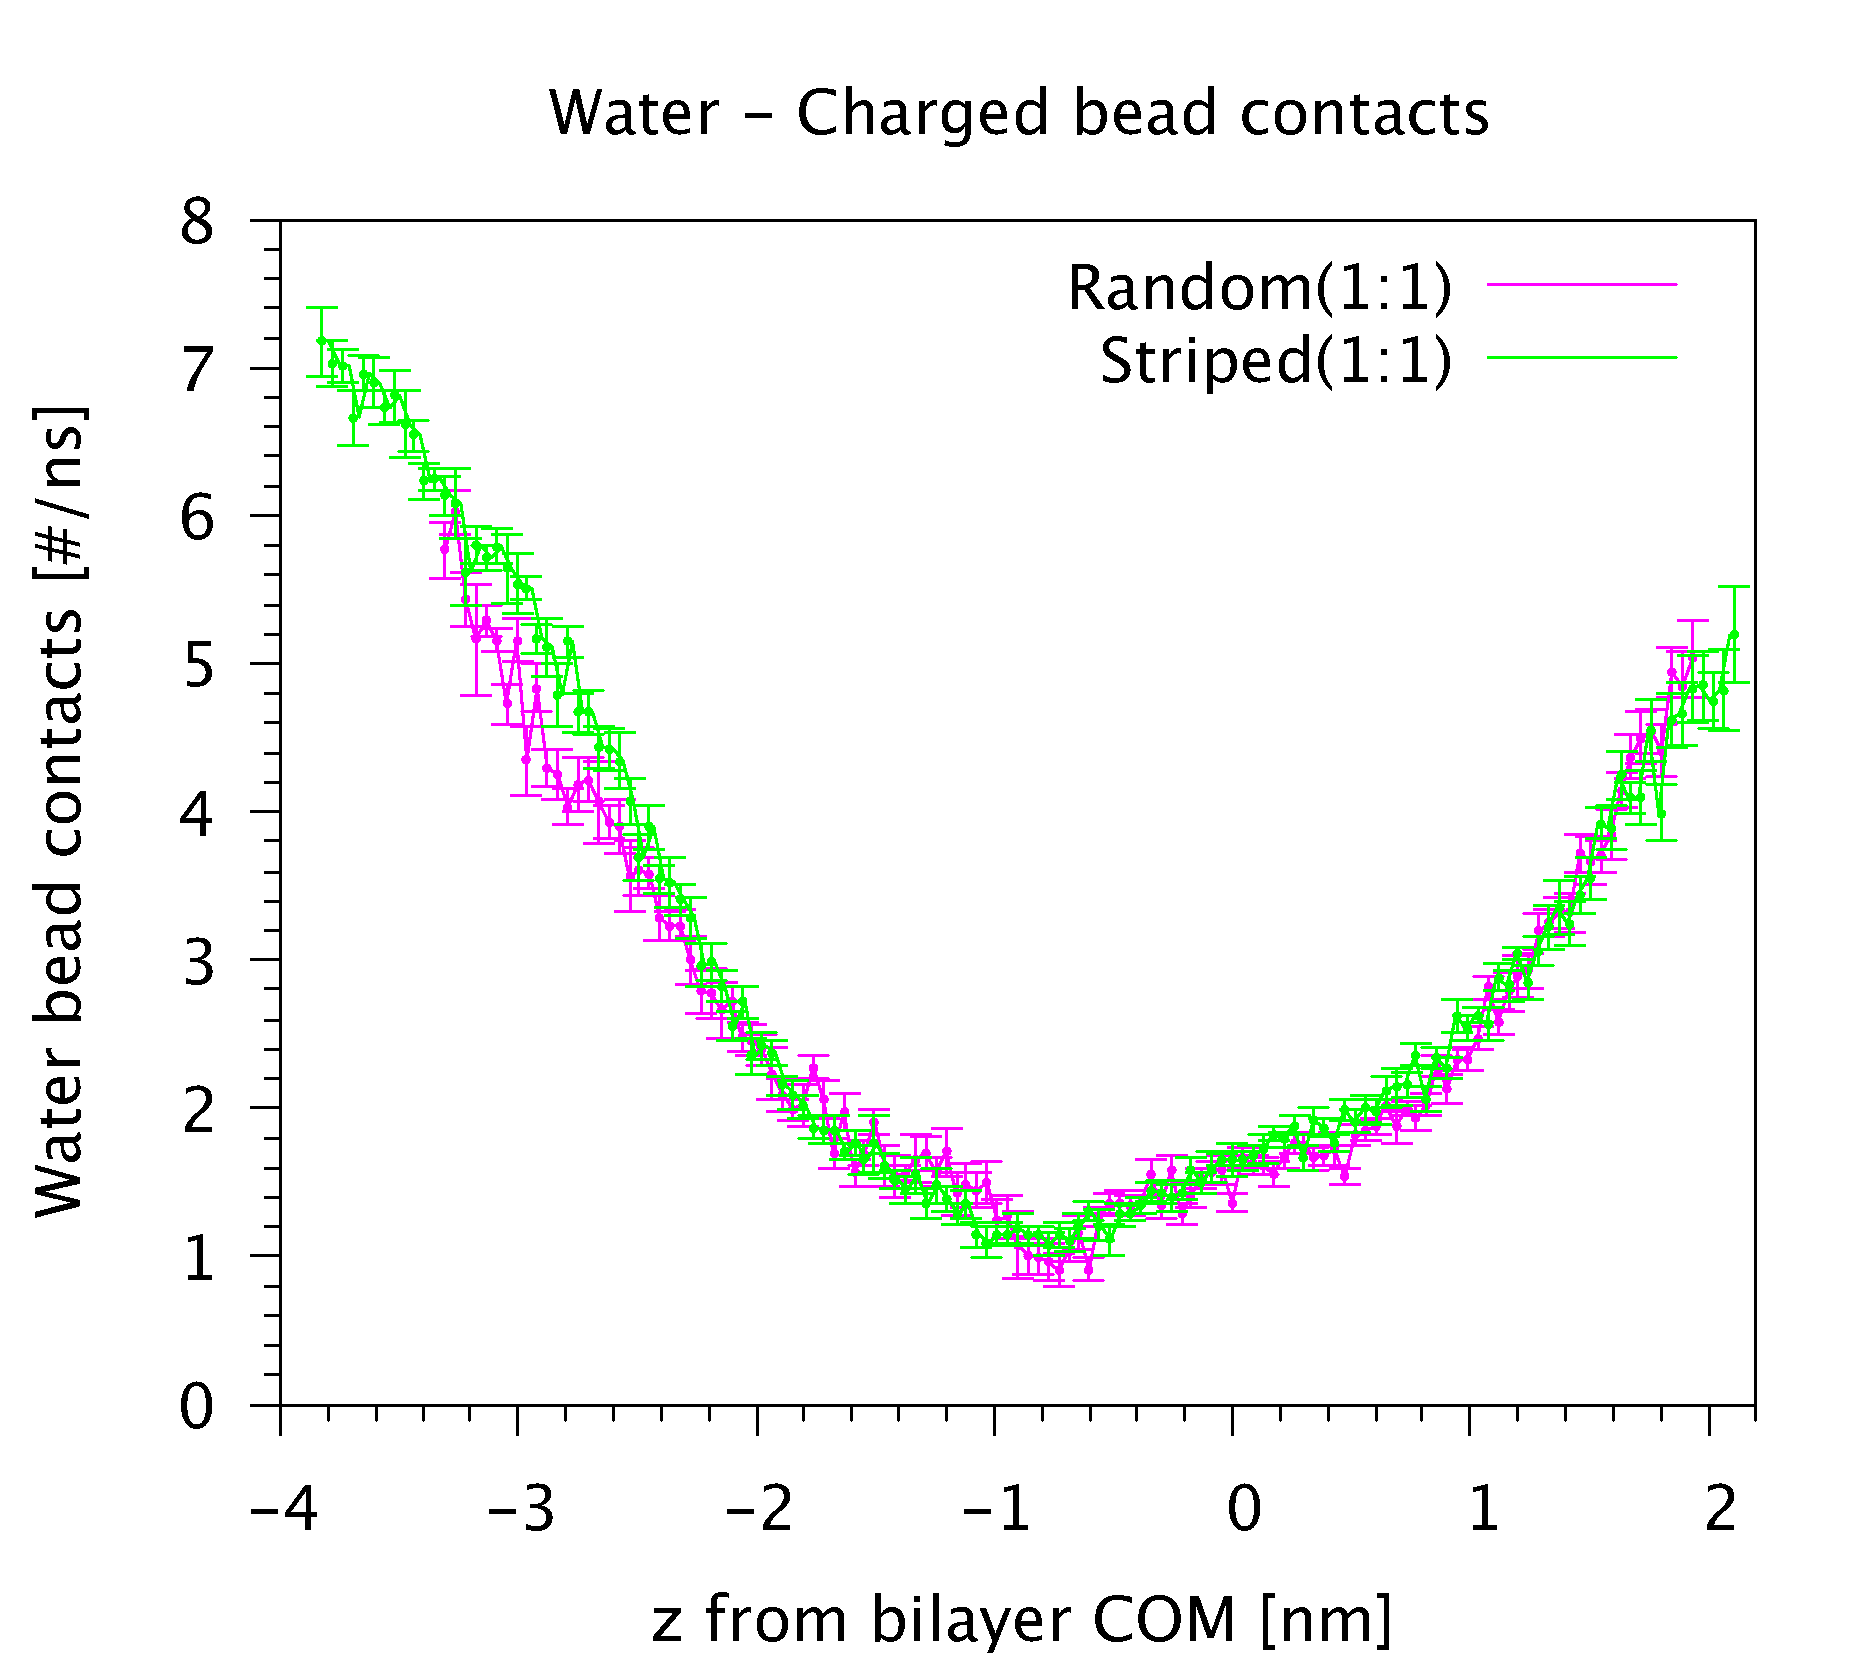
\includegraphics[width=0.5\textwidth]{./img/results/WRPComparison}
	}%
	\caption{Comparison of the contacts per second in function of the time between \acs{PW} beads and the charged bead. (a) comparison between different models. (b) comparison between striped and random \acs{NP}s.}
\end{figure}


\section{Lipid heads dragging}
%Trascinamento delle teste dei lipidi nelle varie salse

% 	minDistPatched			minDistRandom11
\begin{figure}[p]
	\center
	\subfloat[]{
		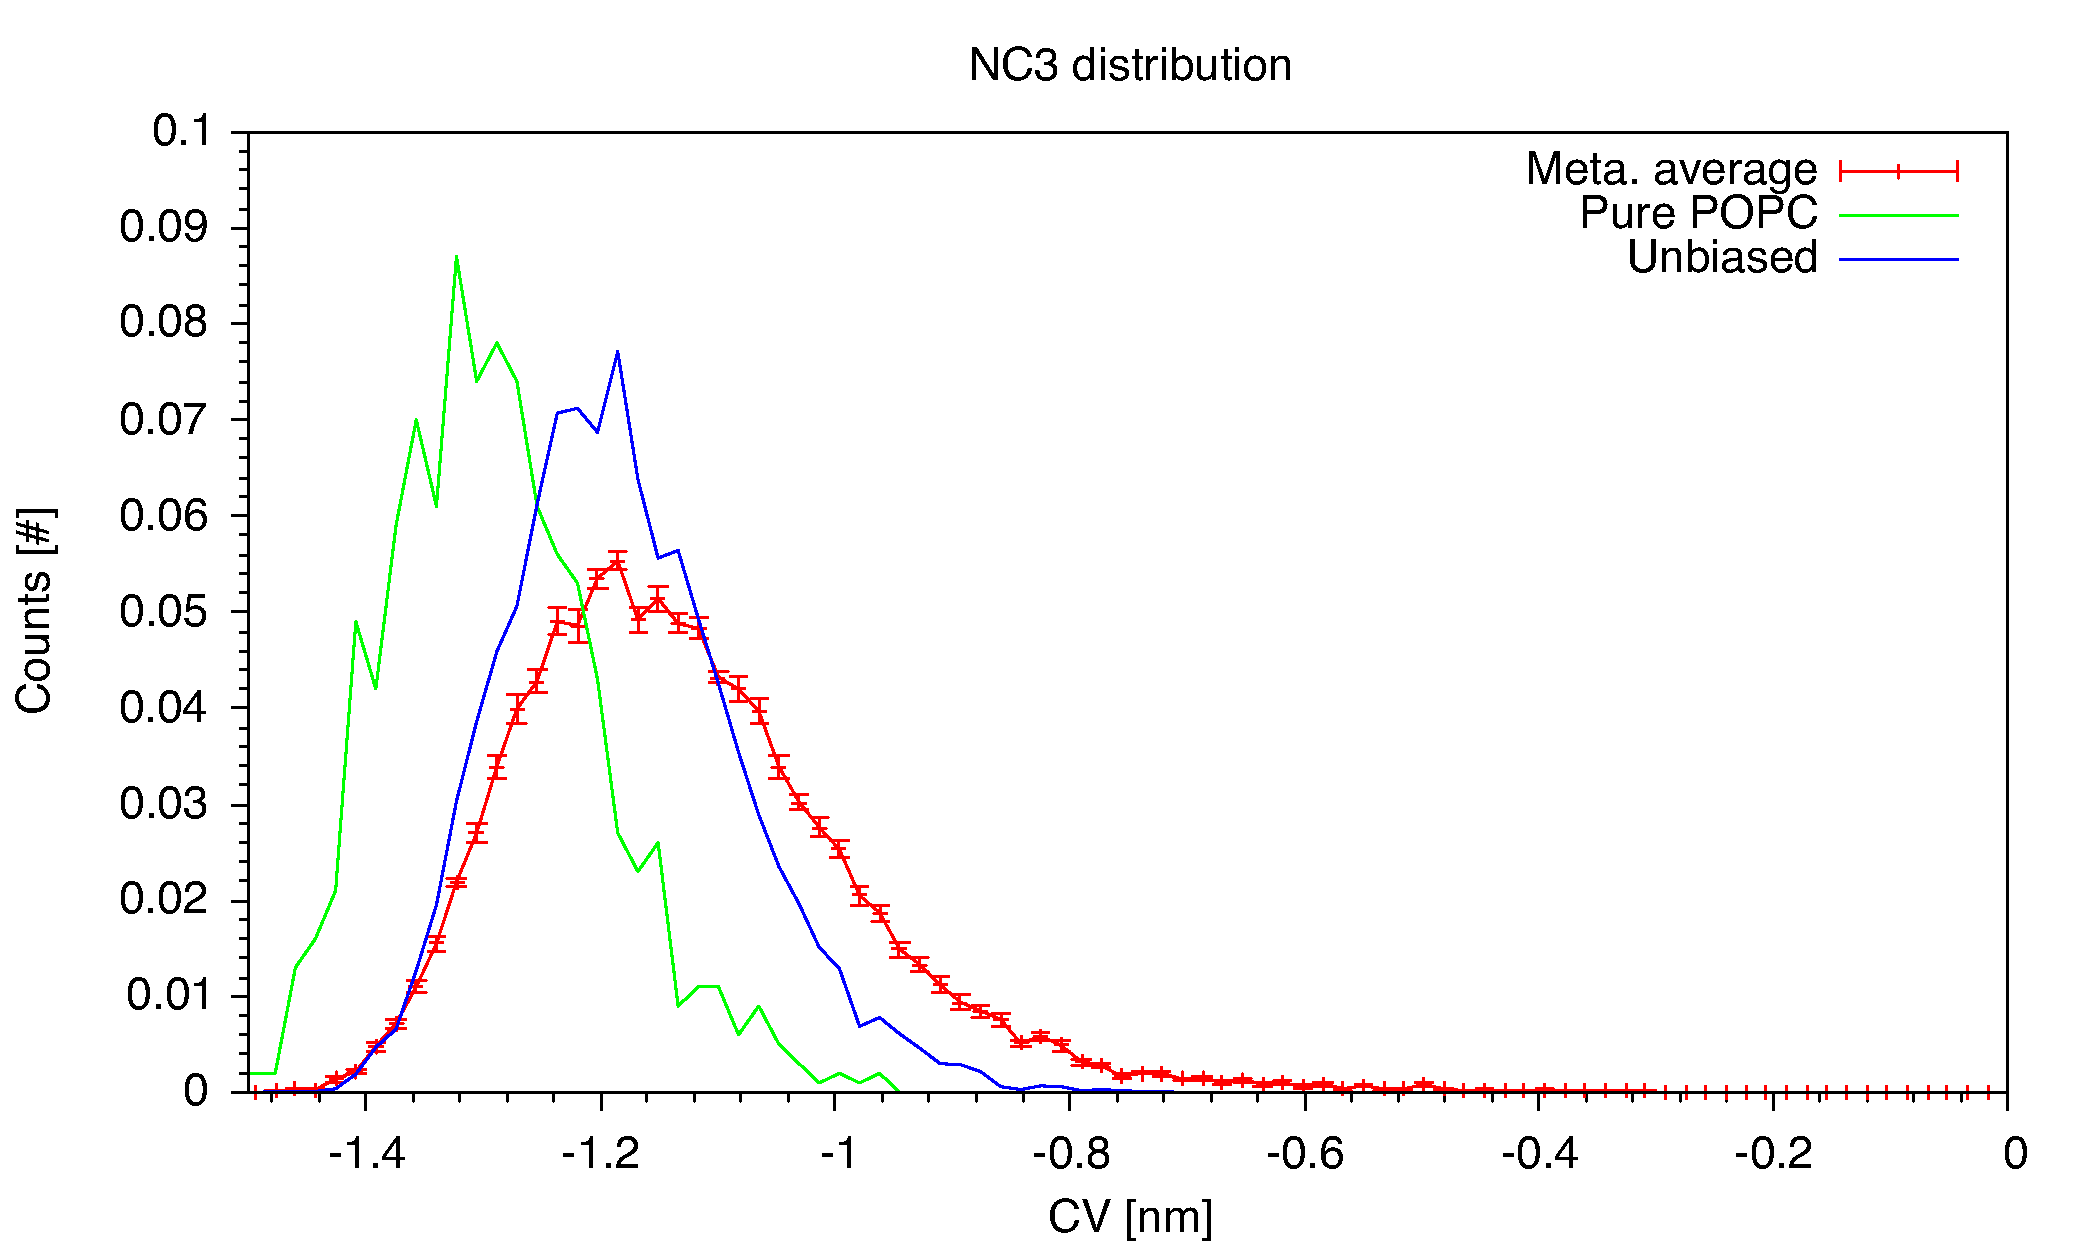
\includegraphics[width=\textwidth]{./img/results/minDistPatched}
	}\\%
	\subfloat[]{
		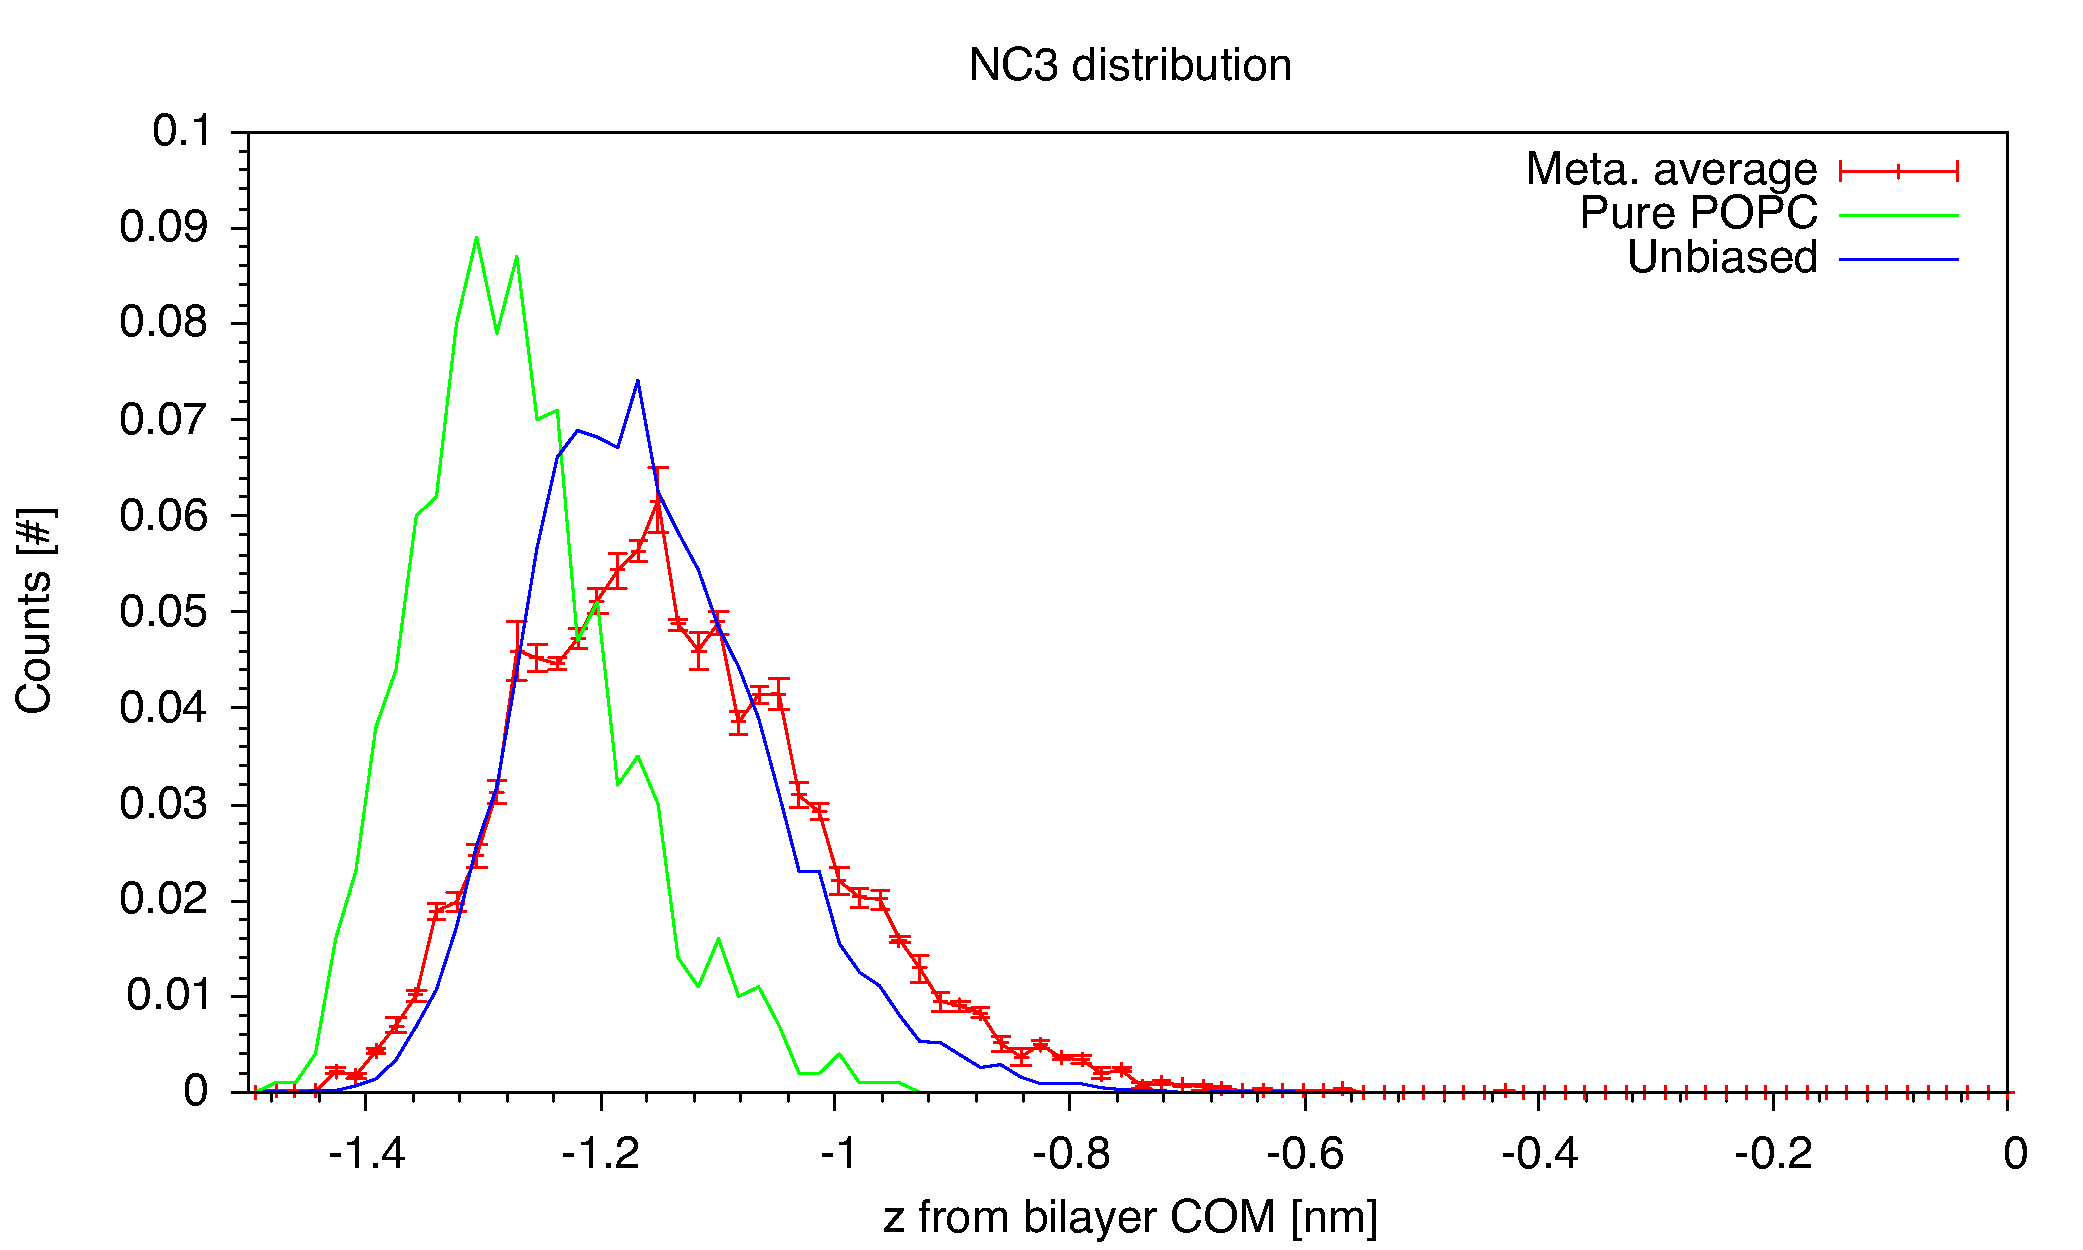
\includegraphics[width=\textwidth]{./img/results/minDistRandom11}
	}%
	\caption{}
\end{figure}

%	NC3PatchedComparison	NC3RPComparison

\section{Effects of metadynamics}
%Quanto la metadinamica sia distrittiva: comparazione tra rum unbiased e biased

% 	minDistHydroPatched		minDistHydroRandom11
\begin{figure}[p]
	\center
	\subfloat[]{
		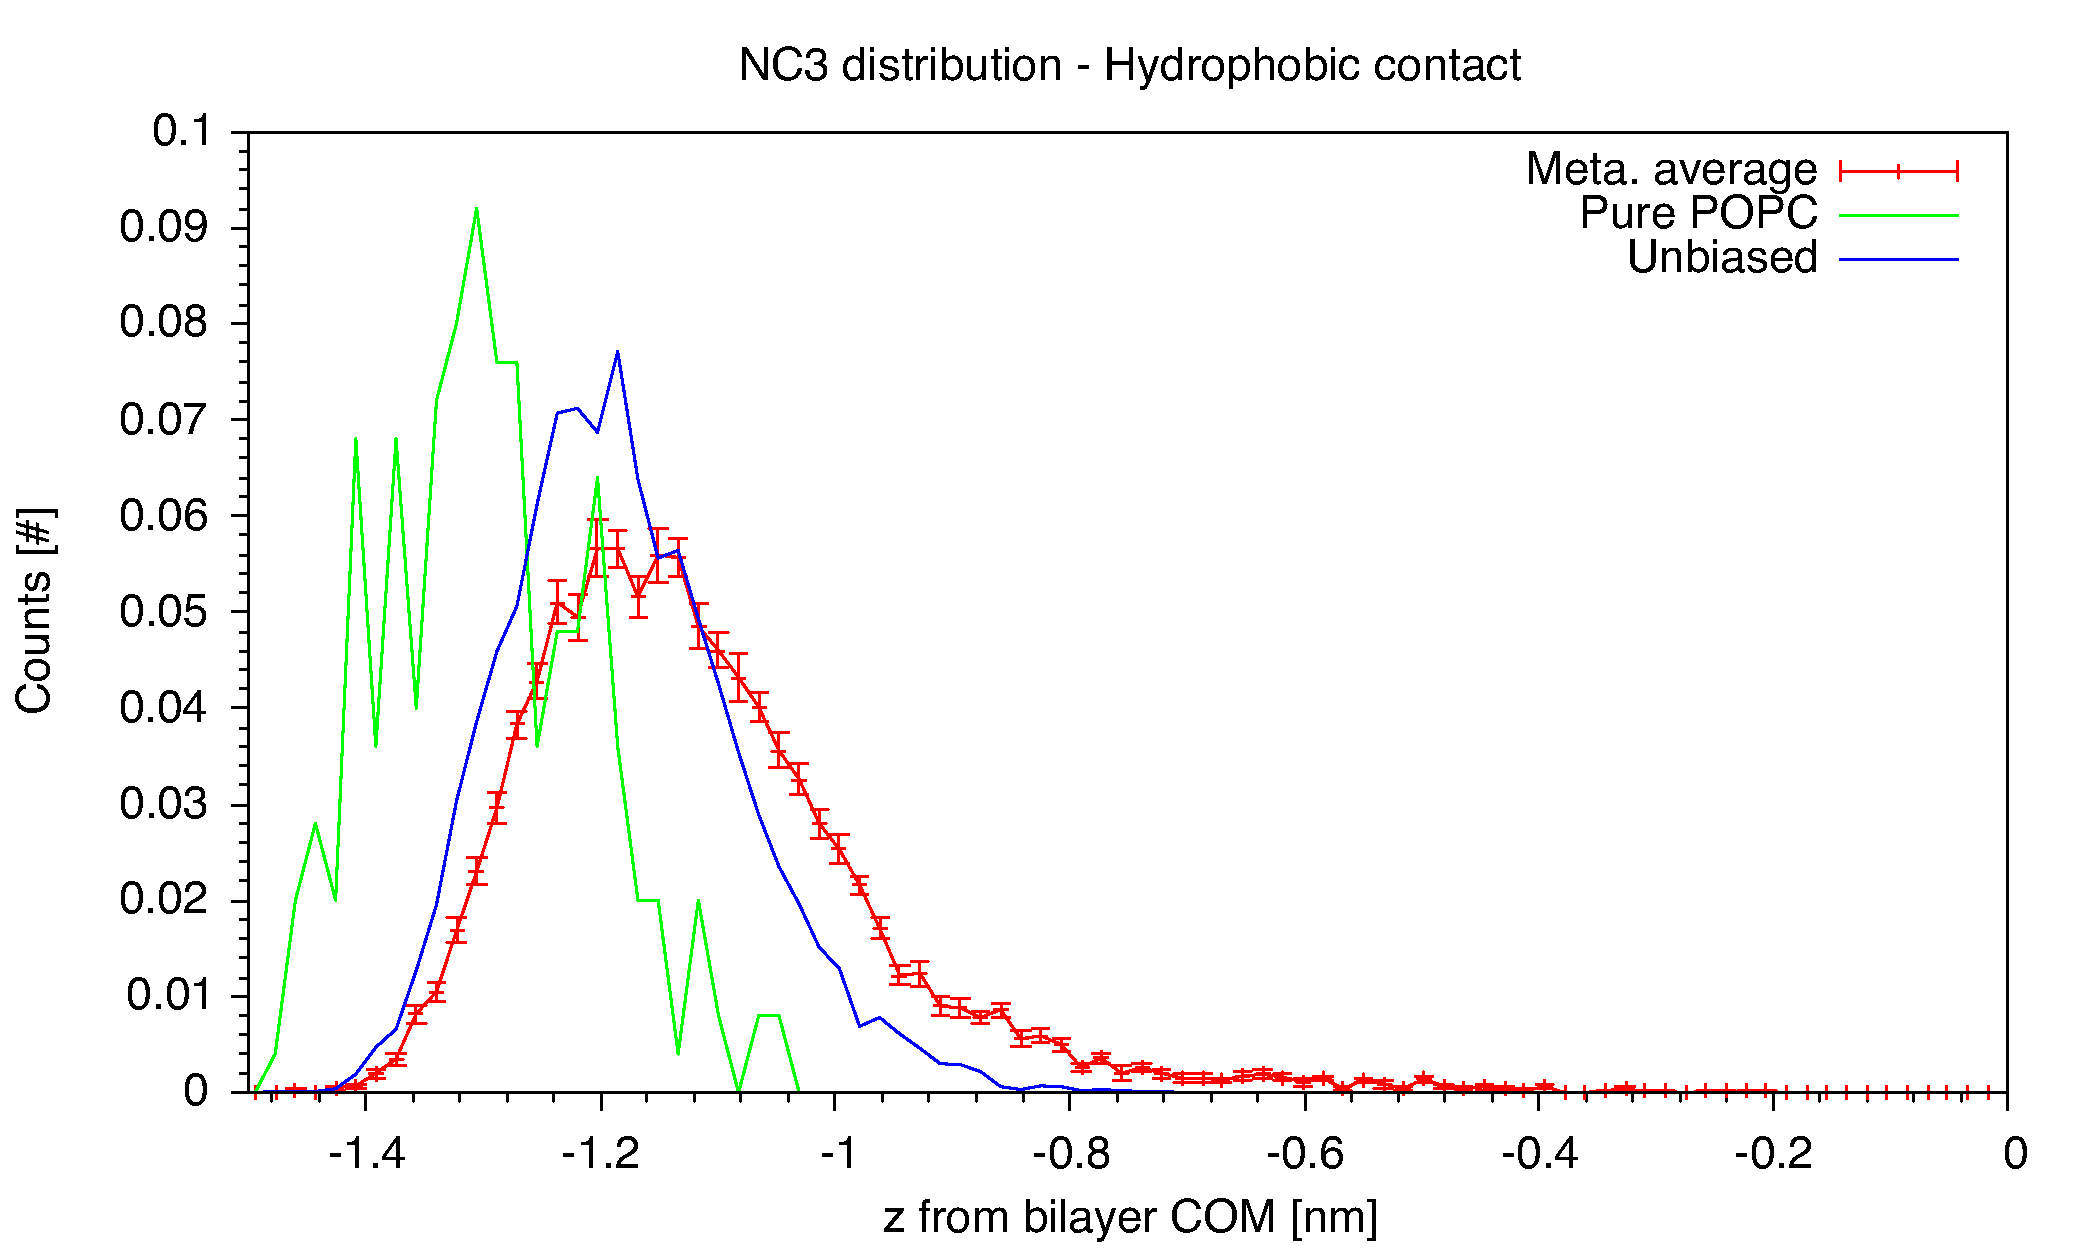
\includegraphics[width=\textwidth]{./img/results/minDistHydroPatched}
	}\\%
	\subfloat[]{
		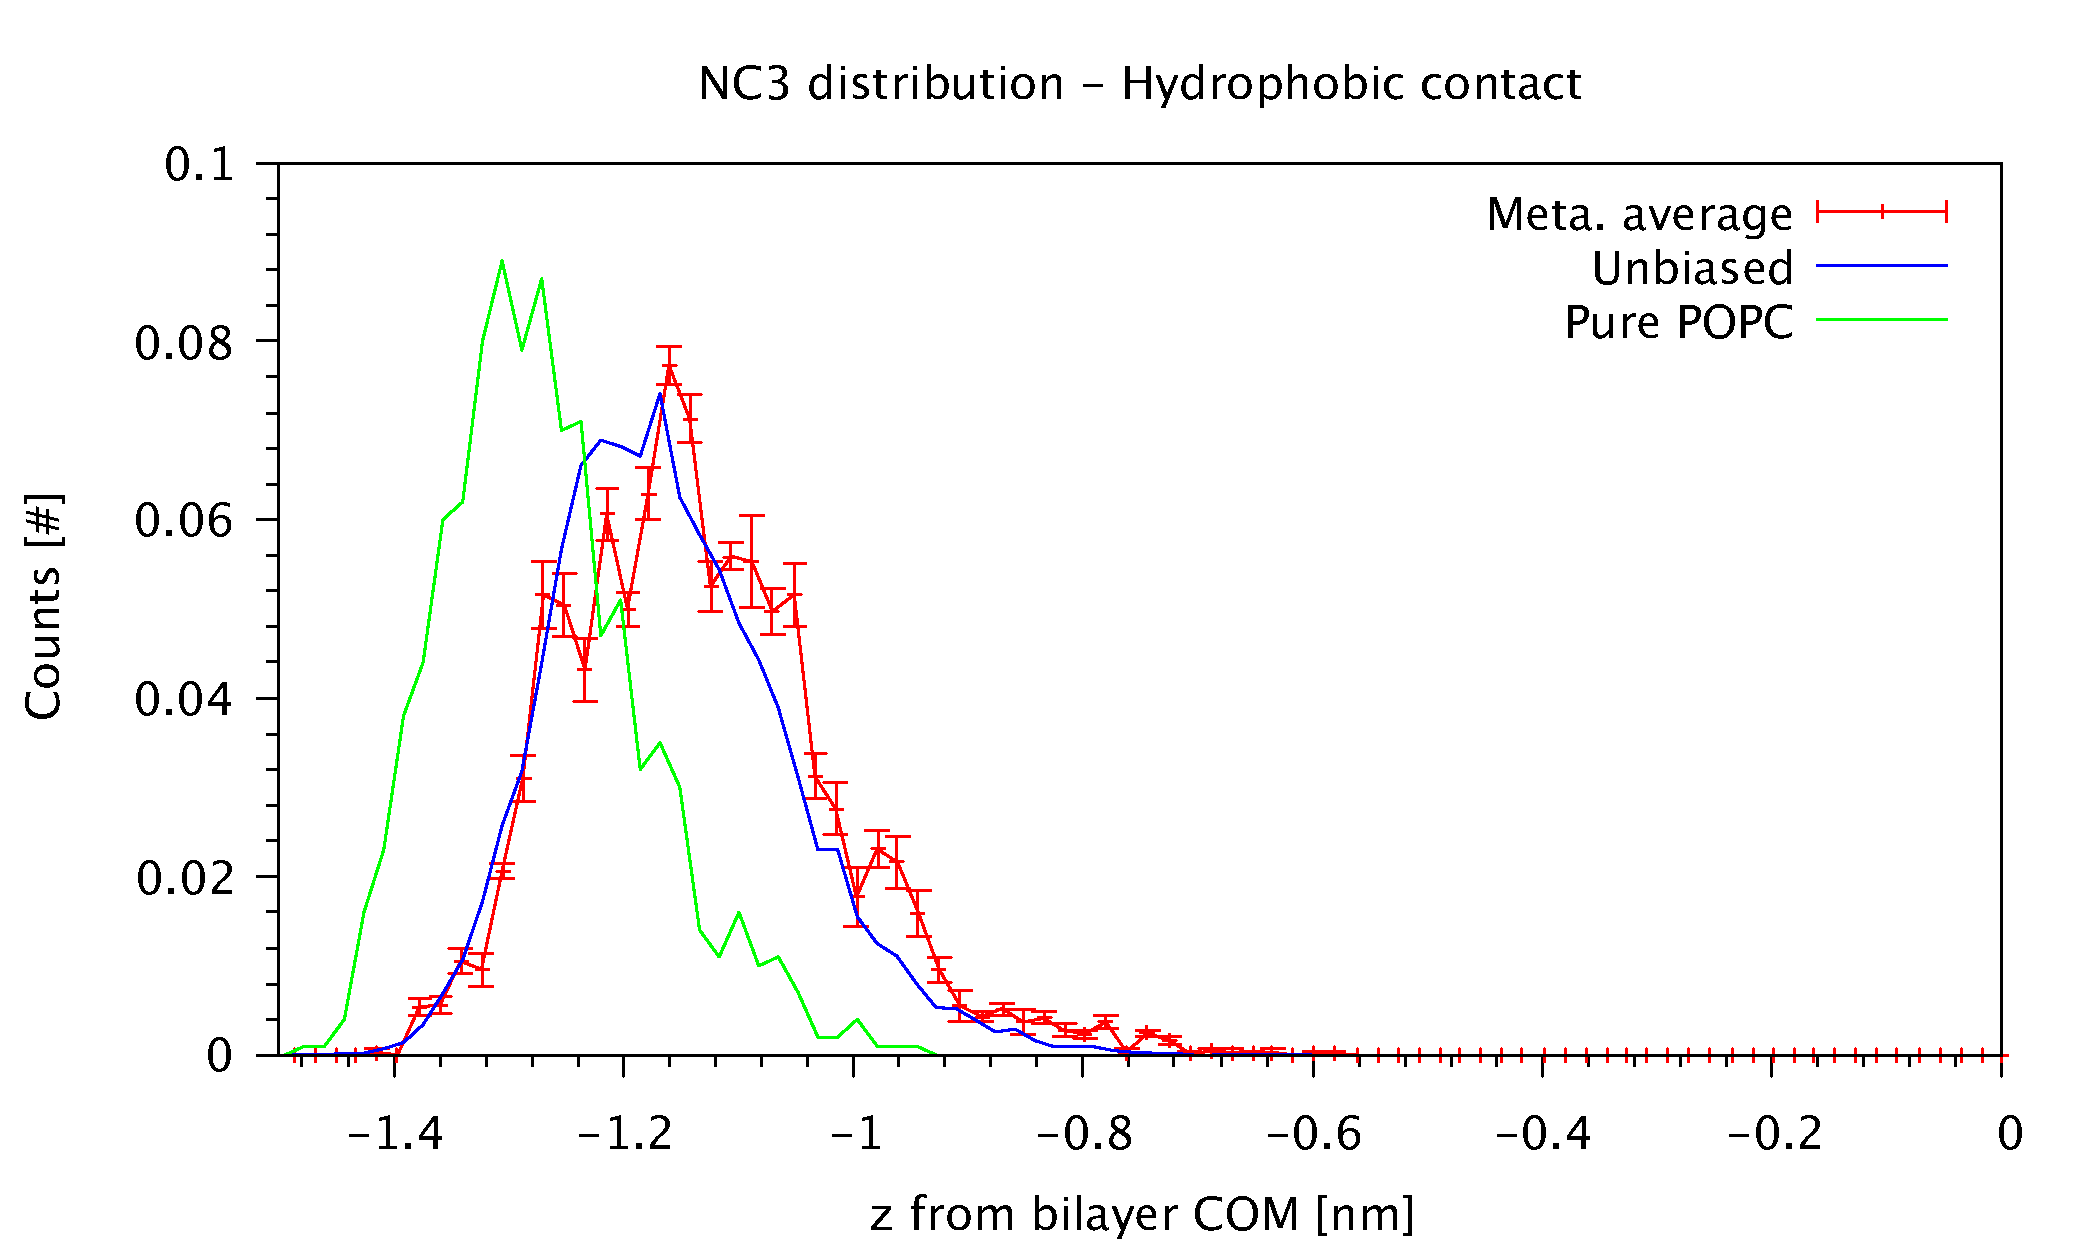
\includegraphics[width=\textwidth]{./img/results/minDistHydroRandom11}
	}%
	\caption{}
\end{figure}

%	patchedPWContact	randon11PWContact
% 	patchedNC3Contact	
\begin{figure}[p]
	\center
	\subfloat[]{
		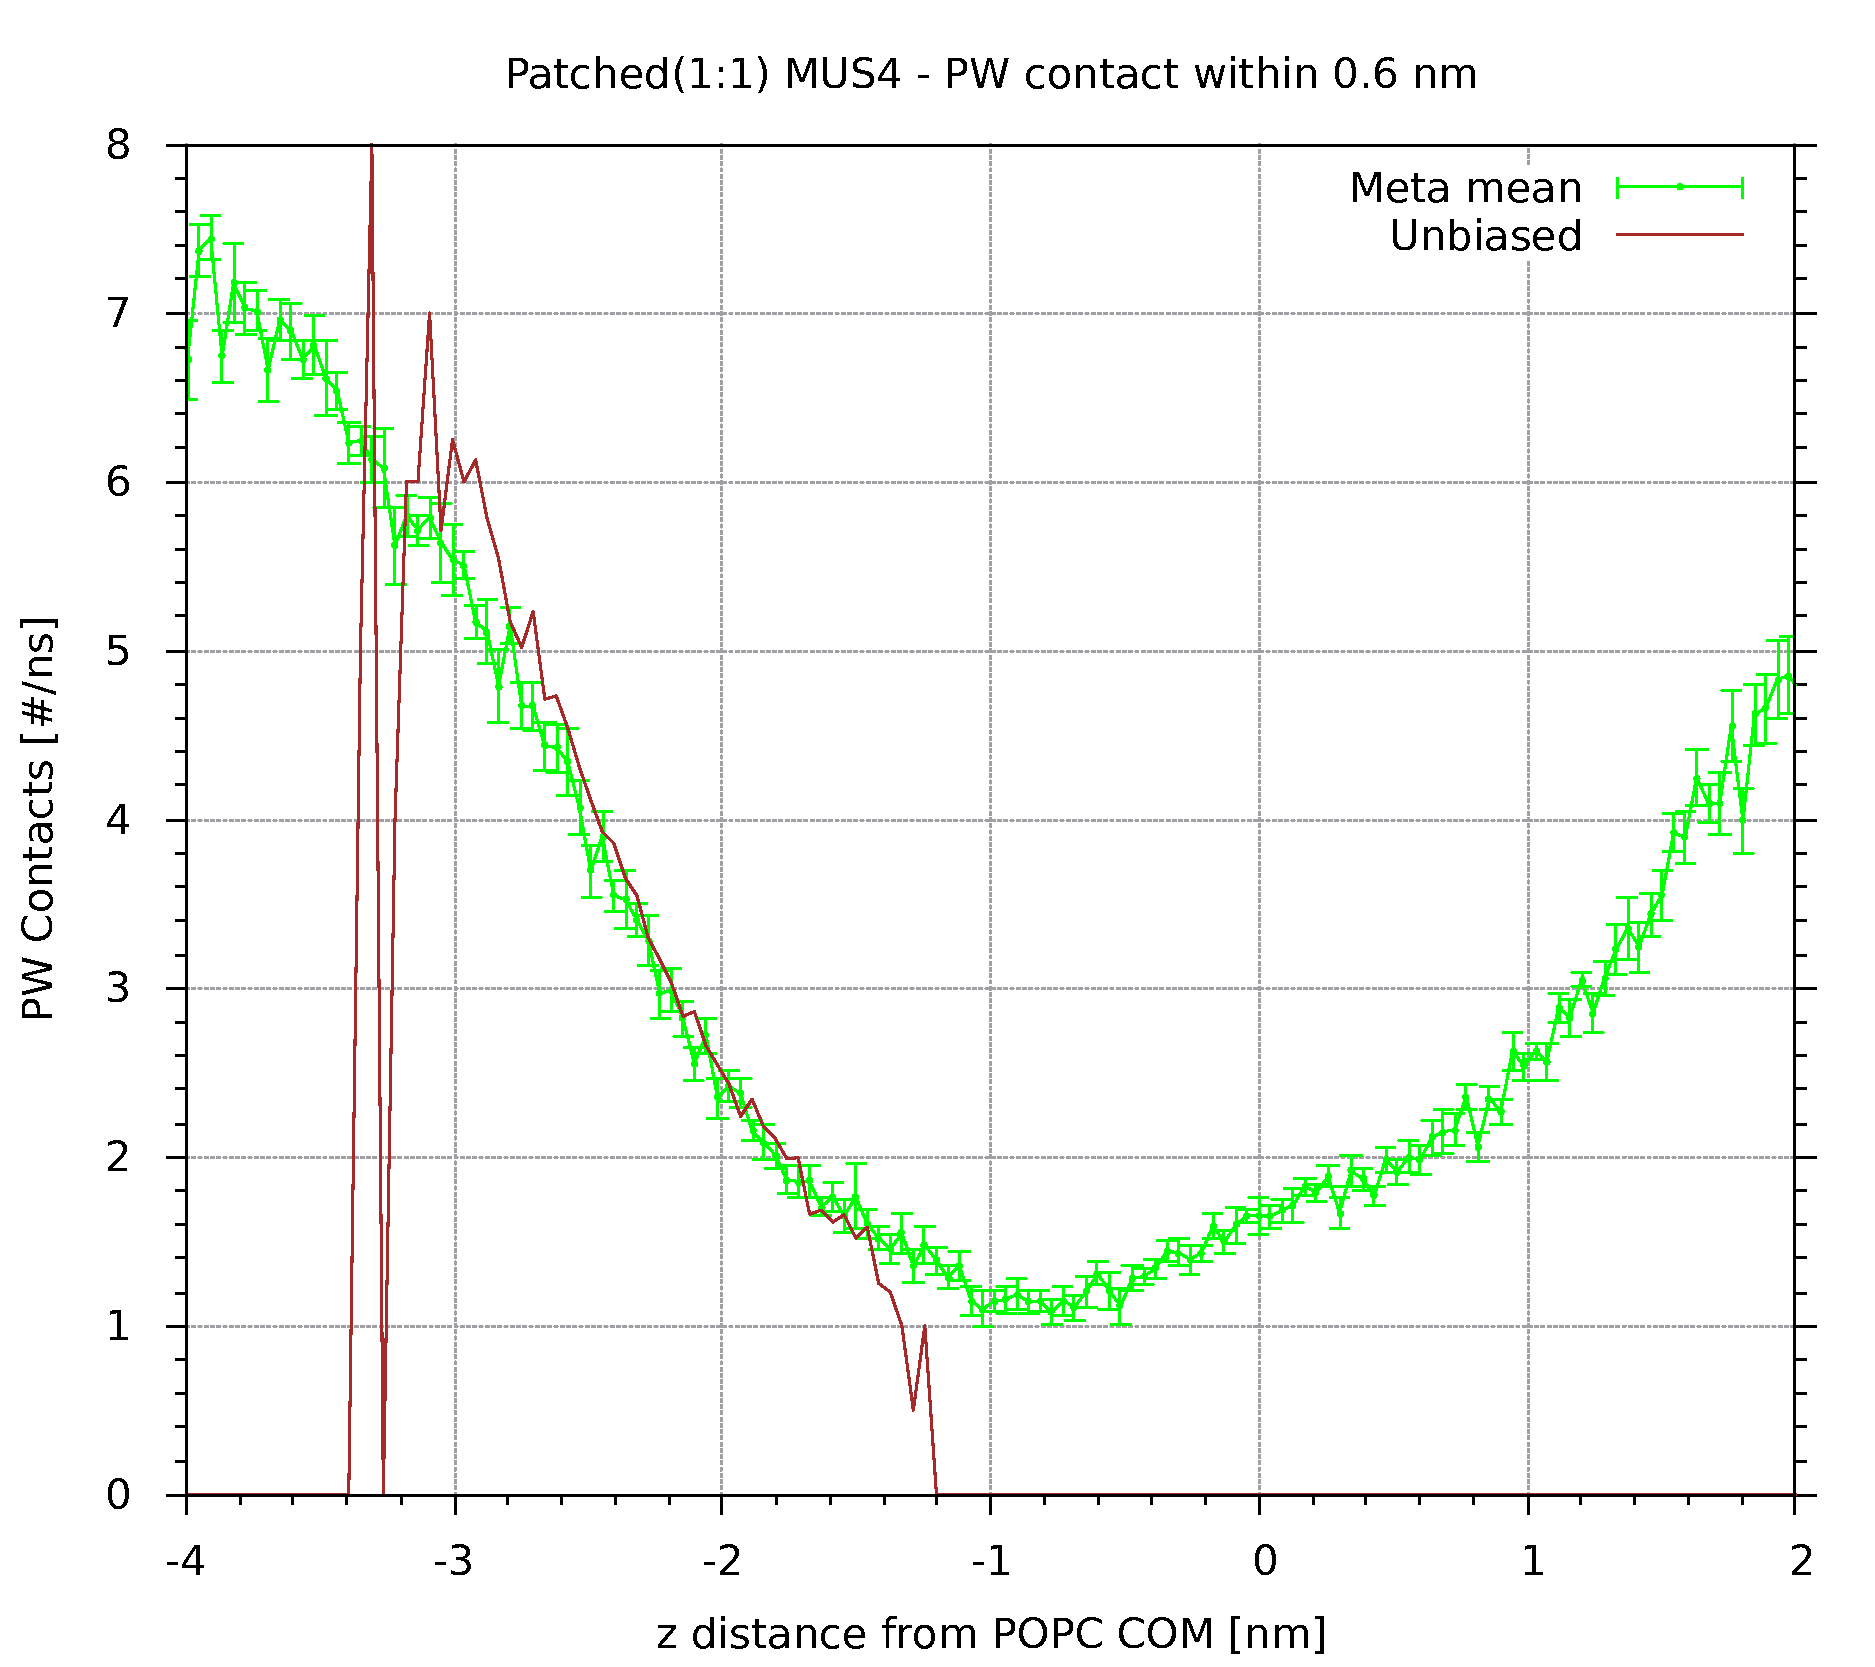
\includegraphics[width=0.5\textwidth]{./img/results/patchedPWContact}
	}%
	\subfloat[]{
		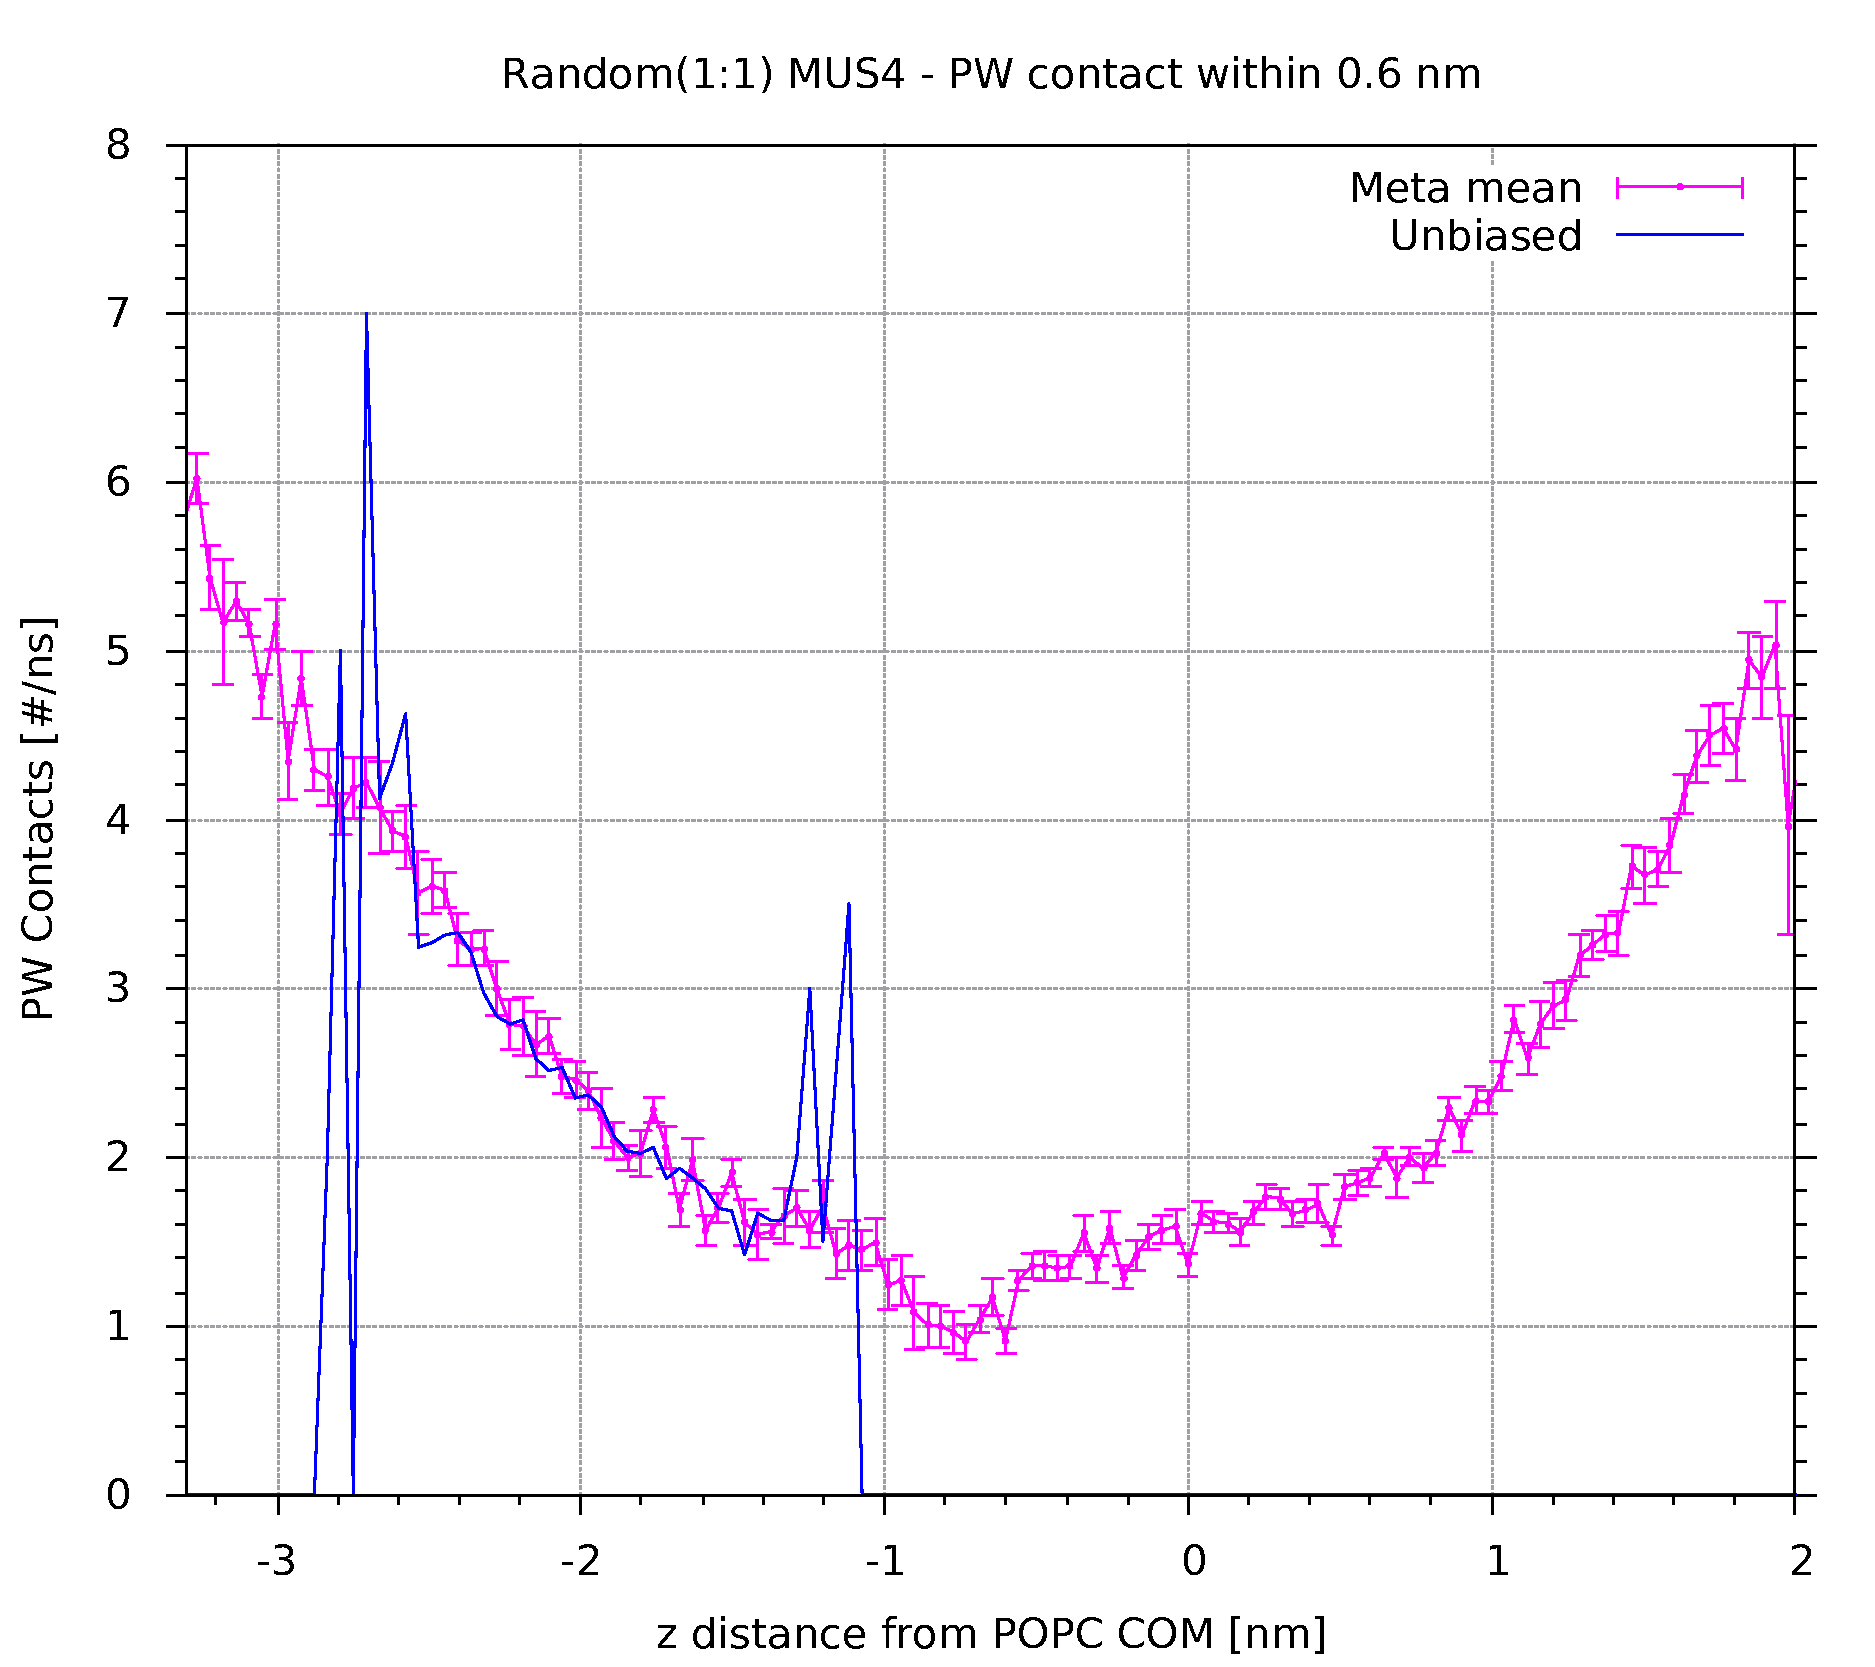
\includegraphics[width=0.5\textwidth]{./img/results/randon11PWContact}
	}\\%
	\subfloat[]{
		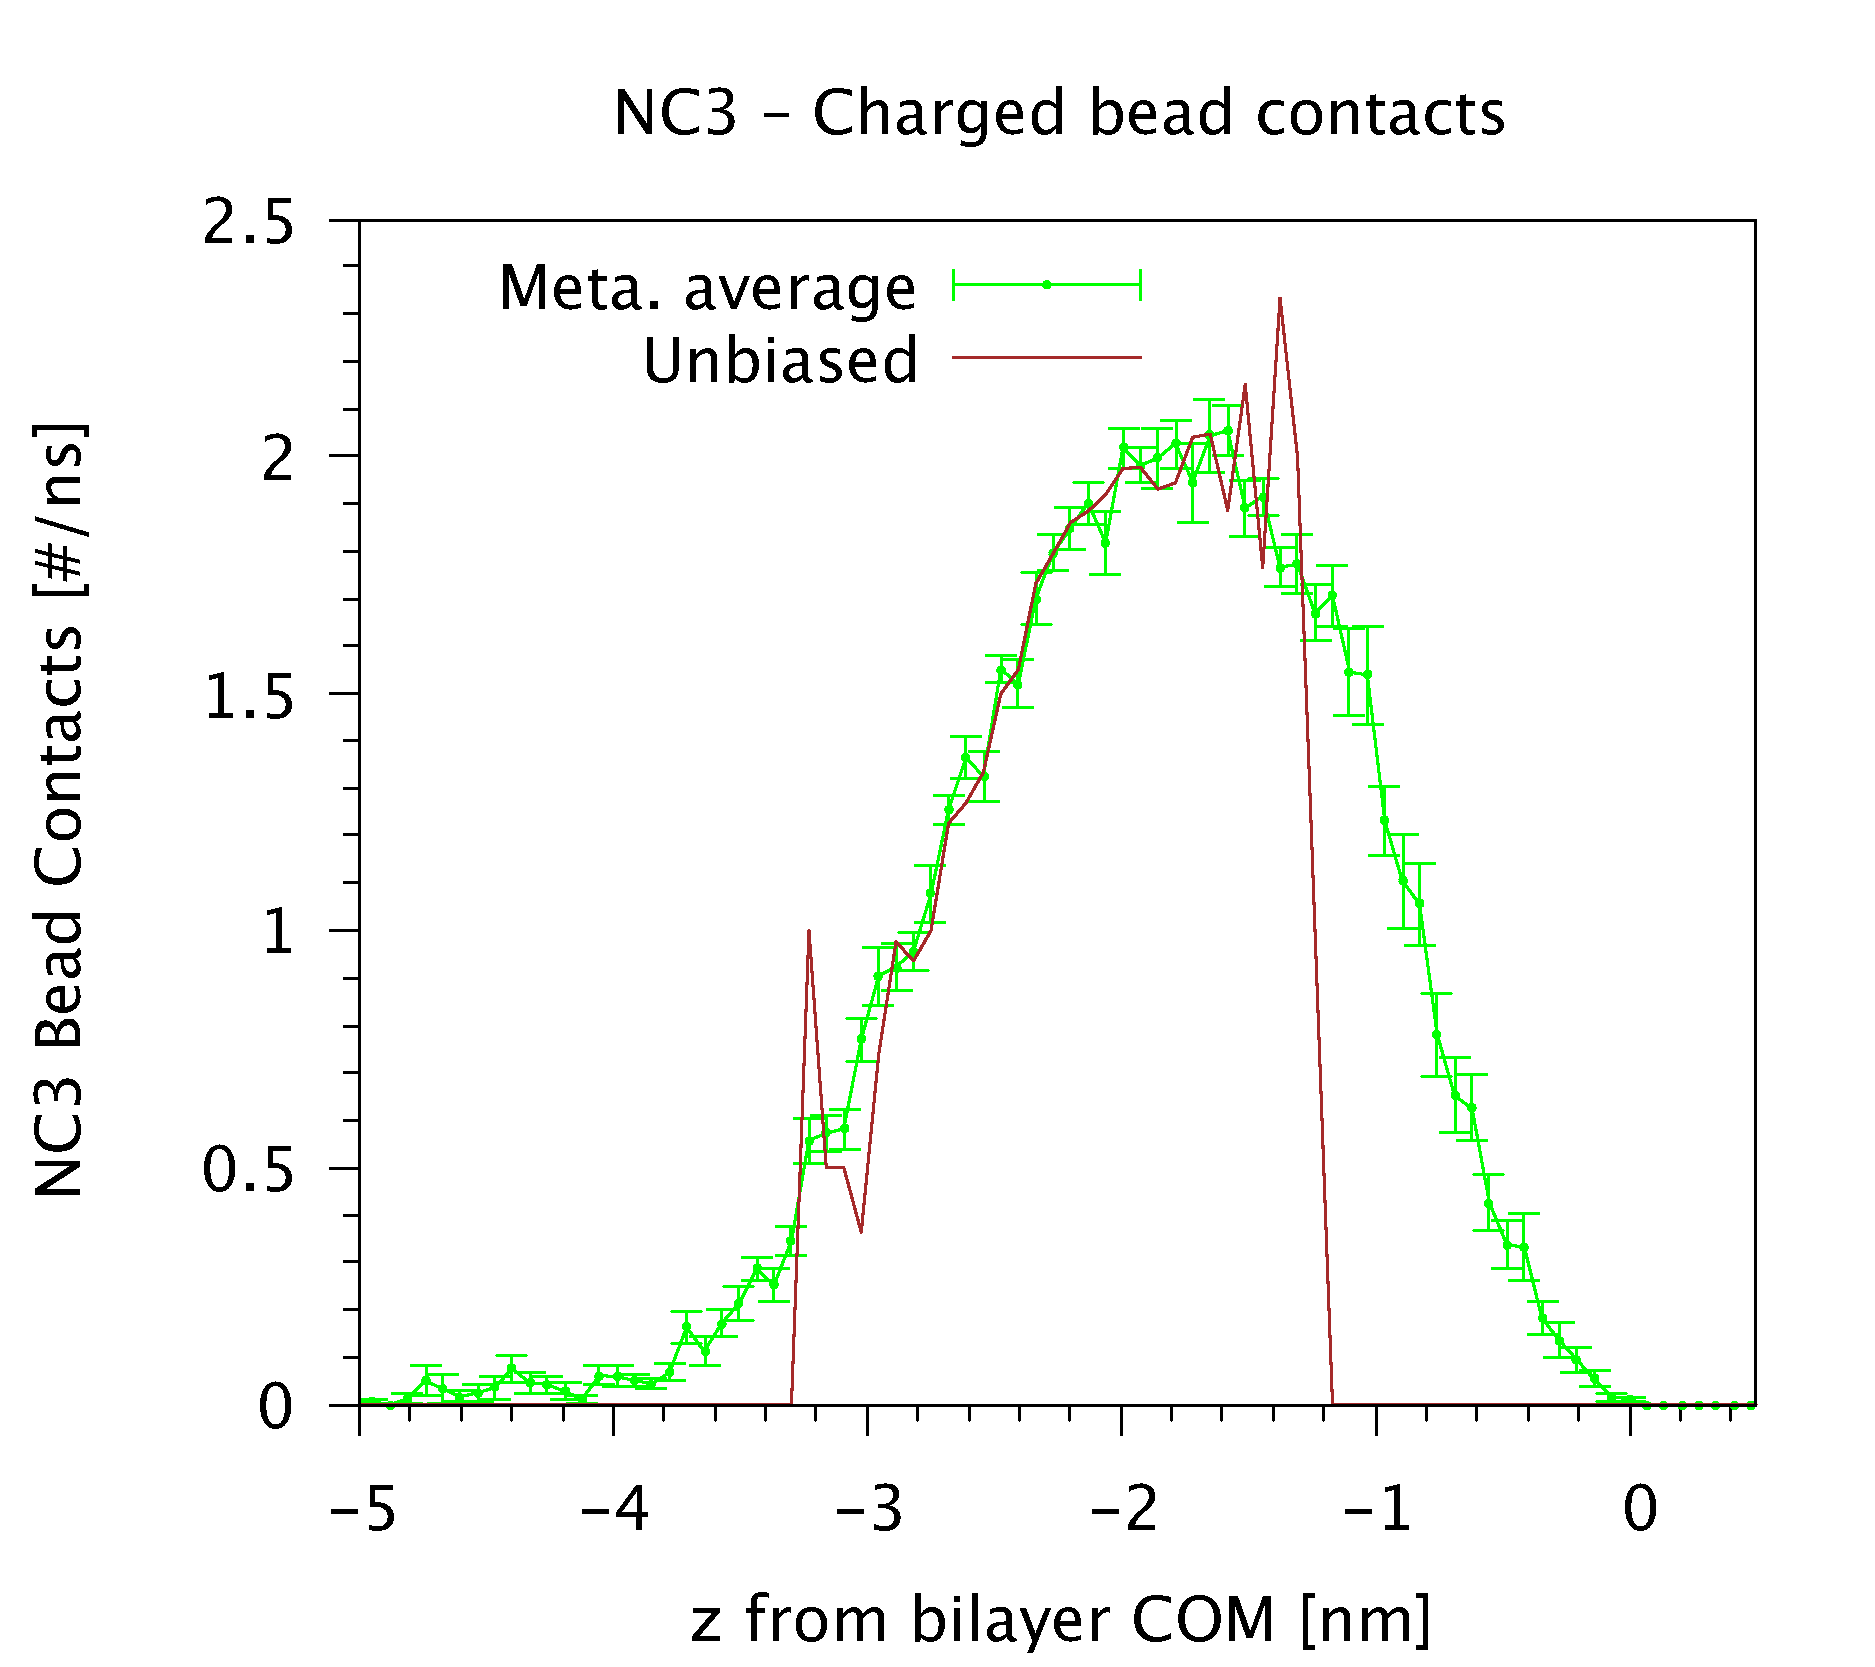
\includegraphics[width=0.5\textwidth]{./img/results/patchedNC3Contact}
	}%
	\subfloat[]{
		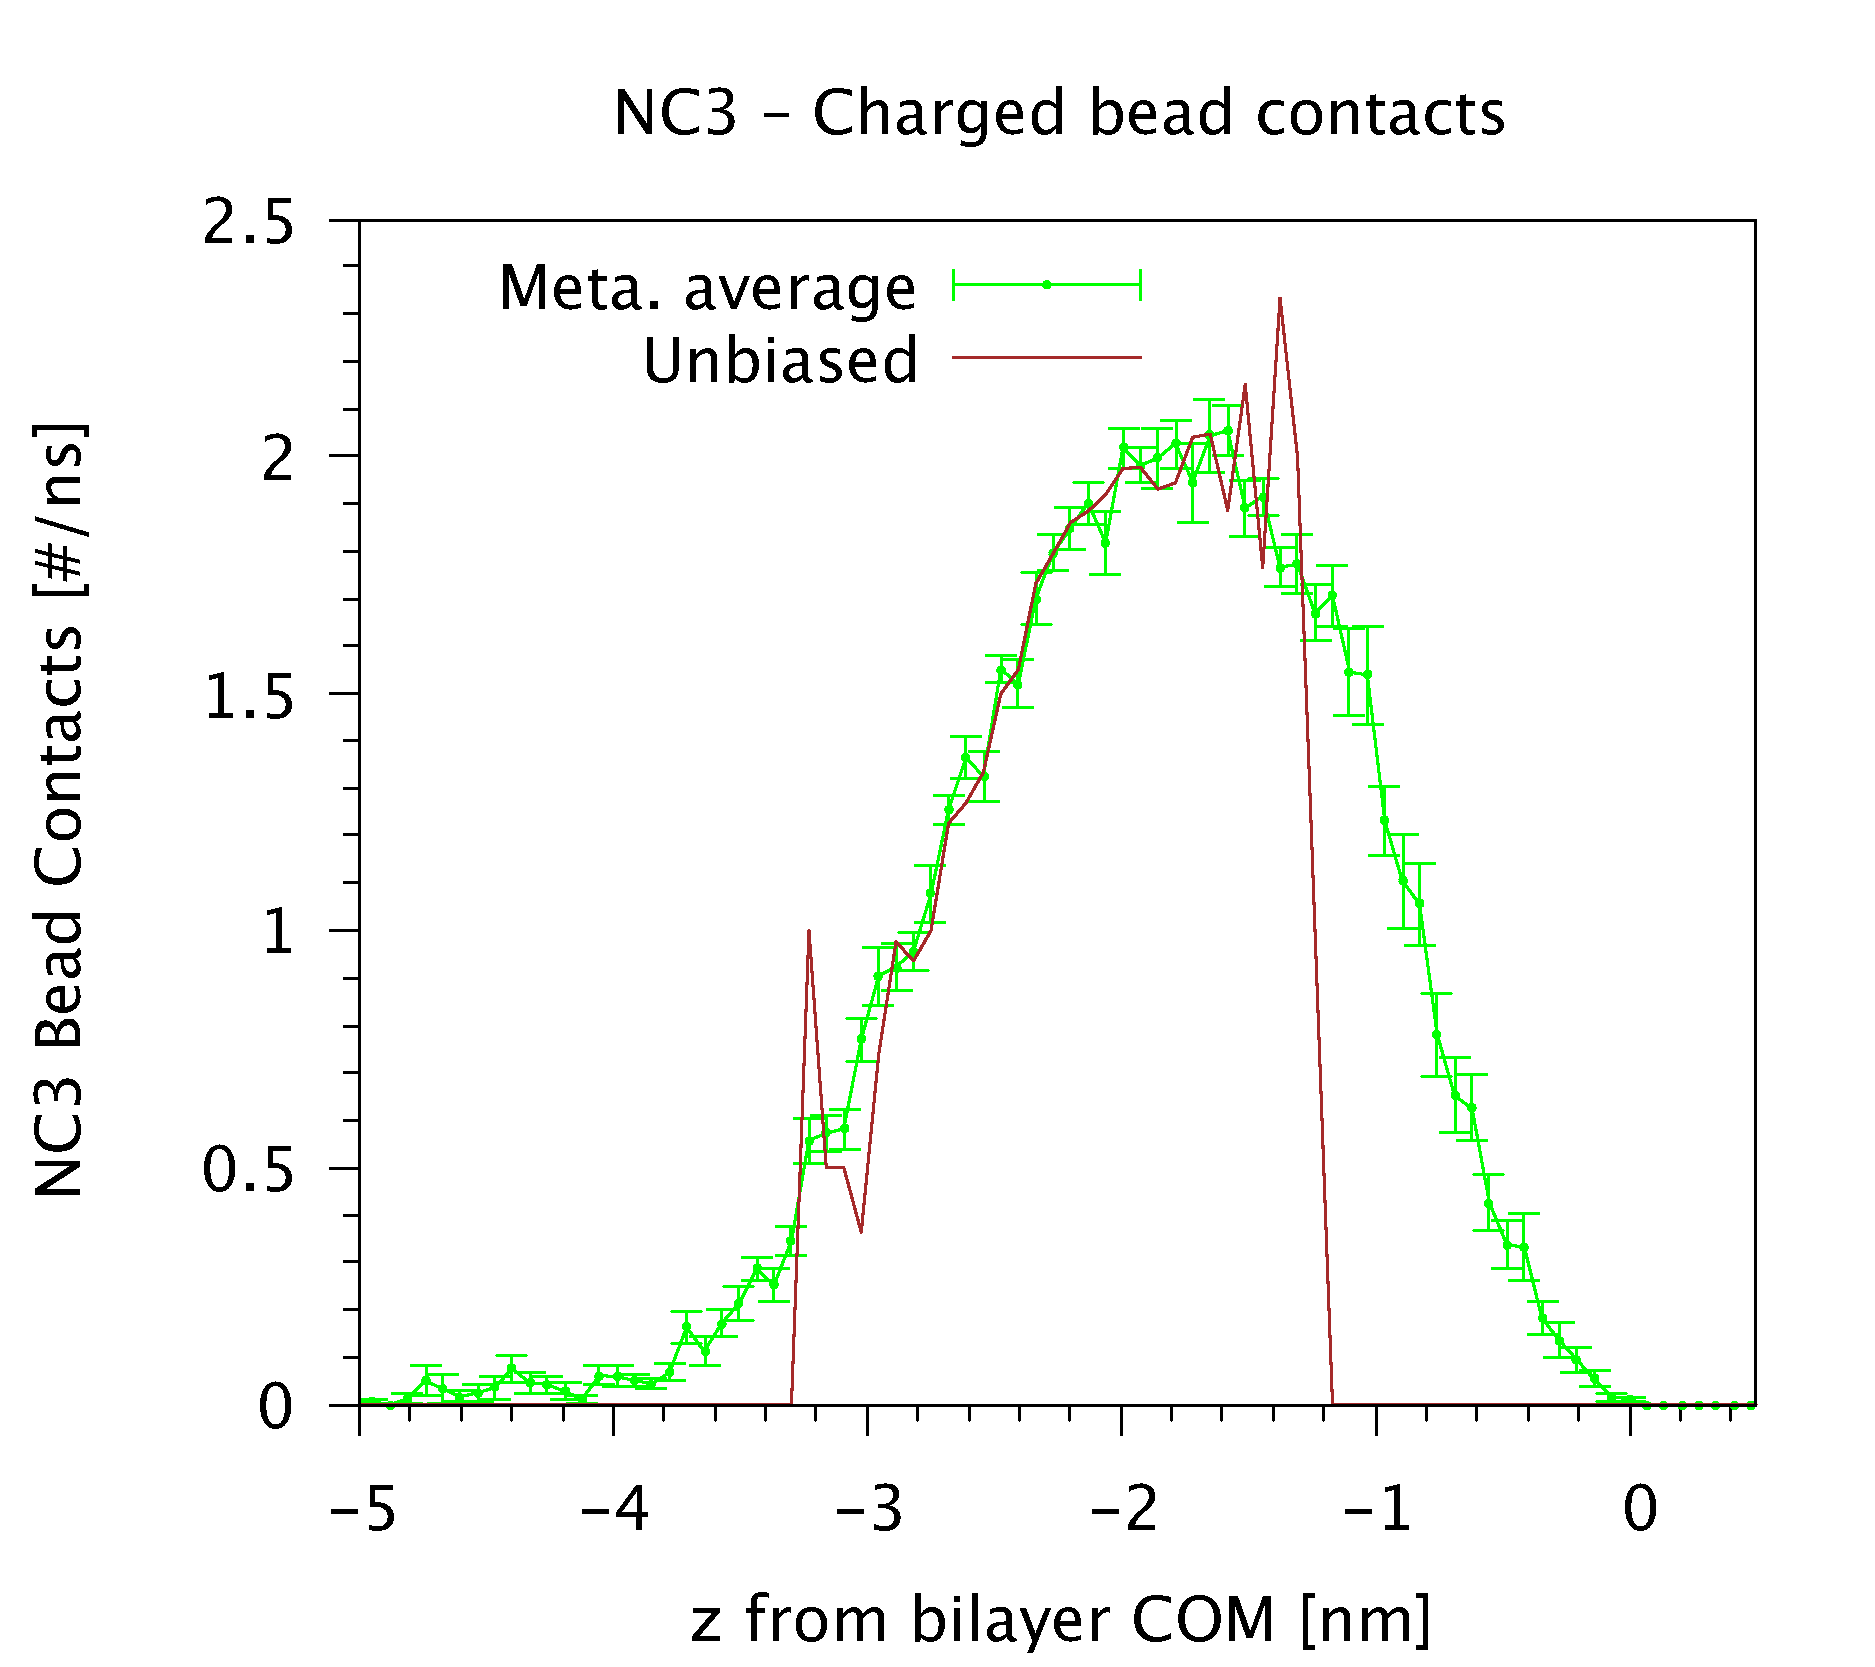
\includegraphics[width=0.5\textwidth]{./img/results/patchedNC3Contact}
	}
	\caption{(a-b) Number of contacts per ns in function of the $z$ component of the distance between the \acs{COM} of the bilayer and the center of the charged bead between the \acs{PW} beads and the charged bead for the \acs{NP} configuration: (a) striped and (b) random. (c-d) The same for the coline group and the charged bead; (c) striped and (d) random. For each plots the number of contacts are in comparison with the corresponding unbiased run.}
\end{figure}


\section{NP and membrane properties}
%Proprietà generali
%Coef di diffusione stato ancorato, stato idrofobico

\begin{table}[h!t]
	\centering
	\begin{tabular}{lccc}
		\toprule
		\,		 & striped($1$:$1$)		& random($1$:$1$)		& random($1$:$2$)					\\ \toprule
		$D^h_{\text{NP}}$ [$10^{-8}$~cm$^2$/s] & $12 \pm 2$ & $5 \pm 2$ & $5.7 \pm 0.7$ 				\\ \midrule
		$D_{tl}$ [$10^{-8}$~cm$^2$/s] & $30 \pm 1$ & $\mathbf{25 \pm 1}$ & $\mathbf{27.8 \pm 0.1}$	\\ \midrule
		$D_{bl}$ [$10^{-8}$~cm$^2$/s] & $\mathbf{22 \pm 2}$ & $27 \pm 3$	& $35 \pm 1$			\\ \midrule
		$\overline{d_z}$ [nm] & $1.996 \pm 0.0016$	& $2.2794 \pm 0.0017$	& $2.7284 \pm 0.0014$	\\ \bottomrule
	\end{tabular}
	\caption{Lateral diffusion coefficients: of the \acs{NP} in the hydrophobic state ($D^h_\text{NP}$), of the lipids in the top leaflet ($D_{tl}$) and in the bottom leaflet ($D_{bl}$). $\overline{d_z}$ is the average $z$ component of the distance between the \acs{COM} of the \acs{NP} and the \acs{COM} of the \acs{POPC} bilayer. The values in bold font refer to the entrance leaflet. Data obtained from my unbiased runs.}
	\label{tab:NPMembProperties}
\end{table}


\section{Structural properties of the bilayer}
%Risucchio delle membrane al recrossing
%Deformazione del leaflet di ancoraggio: RDF e densitymap 2D